% !TEX program = xelatex
% vim:foldmethod=marker:foldmarker=<<<,>>>
\documentclass[compress,aspectratio=169]{beamer}

%<<< Preamble
\usepackage[english]{babel}
\usepackage{metalogo}
\usepackage{listings}
\usepackage{fontspec}
\usepackage{amsmath, amssymb, bm}
\usepackage{stackrel}
\usepackage{tikz}
\usepackage{unicode-math}
\usepackage{subcaption}


\usepackage[theme=nord,charsperline=60,linenumbers]{jlcode}
\usetheme{Nord}

% Uncomment lines bellow for light theme
% \usepackage[charsperline=60,linenumbers]{jlcode}
% \usetheme{Boadilla}

\setmainfont{Roboto}
% \setsansfont{DejaVu Serif}
% \setmonofont{CaskaydiaCove Nerd Font Mono}
\setmonofont{JuliaMono}

\setbeamercolor{mybullet}{use=itemize item.fg,bg=itemize item.fg,fg=itemize item.fg}

\makeatletter
\def\verbatim@nolig@list{}
\newcommand\pin{%
\parbox[t]{10pt}{\raisebox{0.2pt}{\usebeamercolor[fg]{mybullet}{$\ast$}}}}
\makeatother

\newcommand{\E}[1]{\ensuremath{E\left\{#1\right\}}}
\newcommand{\norm}[1]{\ensuremath{\lVert#1\rVert}}
\newcommand*{\thead}[1]{\multicolumn{1}{c}{\fseries #1}}

\newfontfamily\tabulartext[SizeFeatures={Size=6}]{Roboto}

\hypersetup{
    colorlinks=true,
    urlcolor=NordBlue
}

\DeclareMathOperator*{\argmax}{argmax}
\DeclareMathOperator*{\Var}{Var}
\DeclareMathOperator*{\test}{\gtrless}

\AtBeginDocument{
    \fontsize{8}{12}
    \selectfont

}

\AtBeginSection[]
{
    \begin{frame}[c,noframenumbering,plain]
        \tableofcontents[sectionstyle=show/hide,subsectionstyle=show/show/hide]
    \end{frame}
}


\AtBeginSubsection[]
{
    \begin{frame}[c,noframenumbering,plain]
        \tableofcontents[sectionstyle=show/hide,subsectionstyle=show/shaded/hide]
    \end{frame}
}
%>>>

\title{Project II}
\subtitle{High-Resolution Beamforming on farfield monochromatic signals}
\author{Simon Andreas Bjørn}
\date{April 13, 2023}

\begin{document}

\begin{frame}[plain,noframenumbering]
    \maketitle
\end{frame}

\begin{frame}[fragile] % <<< Estimating the spatial correlation matrix
    \frametitle{Estimating the spatial correlation matrix}
    We want to estimate the spatial correlation matrix from the data generated
    by \jlinl{generate_data.jl}
    \begin{columns}
        \begin{column}{0.5\textwidth}
            \begin{itemize}
                \item Find the spatial correlation matrix by definition
            \end{itemize}
            \begin{jllisting}[gobble=16]
                R = x*x' / N
                heatmap!(ax, abs.(R))
            \end{jllisting}
        \end{column}
        \begin{column}{0.5\textwidth}
            \begin{figure}
                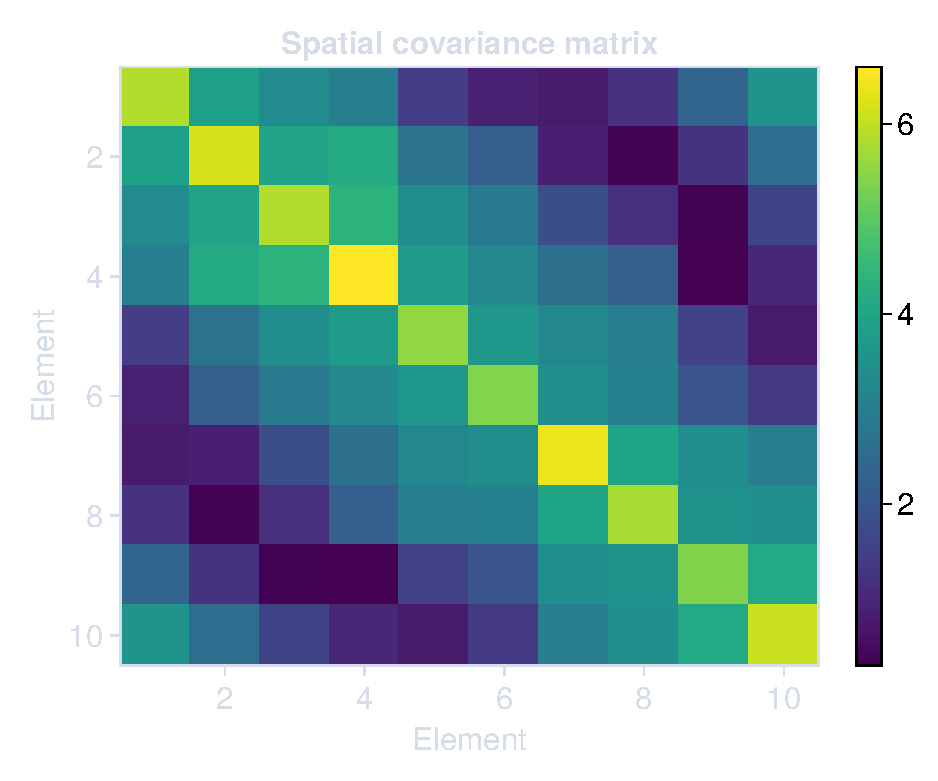
\includegraphics[width=\columnwidth]{"../a.pdf"}
            \end{figure}
        \end{column}
    \end{columns}
\end{frame} 
% >>>

\begin{frame}[fragile] % <<< Estimate spatial spectrum
    \frametitle{Estimate spatial spectrum}
    We now want to estimate the classical spatial spectrum
    \begin{columns}
        \begin{column}{0.4\textwidth}
            \begin{itemize}
                \item We implement functions for the phase factor, steering
                    vector and DAS.
                \item Apply \jlinl{P_DAS} to every angle in DOA
            \end{itemize}
            \begin{jllisting}[gobble=16]
                # Define functions
                DOA  = -40°:0.25°:50°
                ϕ(θ) = -k*d*sin.(θ)
                a(θ) = @. exp(1im*ϕ(θ)*(0:M-1))
                P_DAS(θ) = (a(θ)'*R*a(θ)) / M

                # Apply on DAS
                P_BF = @. abs(P_DAS(DOA))^2
                # Normalize
                P_BF ./= maximum(P_BF);
            \end{jllisting}
        \end{column}
        \begin{column}{0.6\textwidth}
            \begin{figure}
                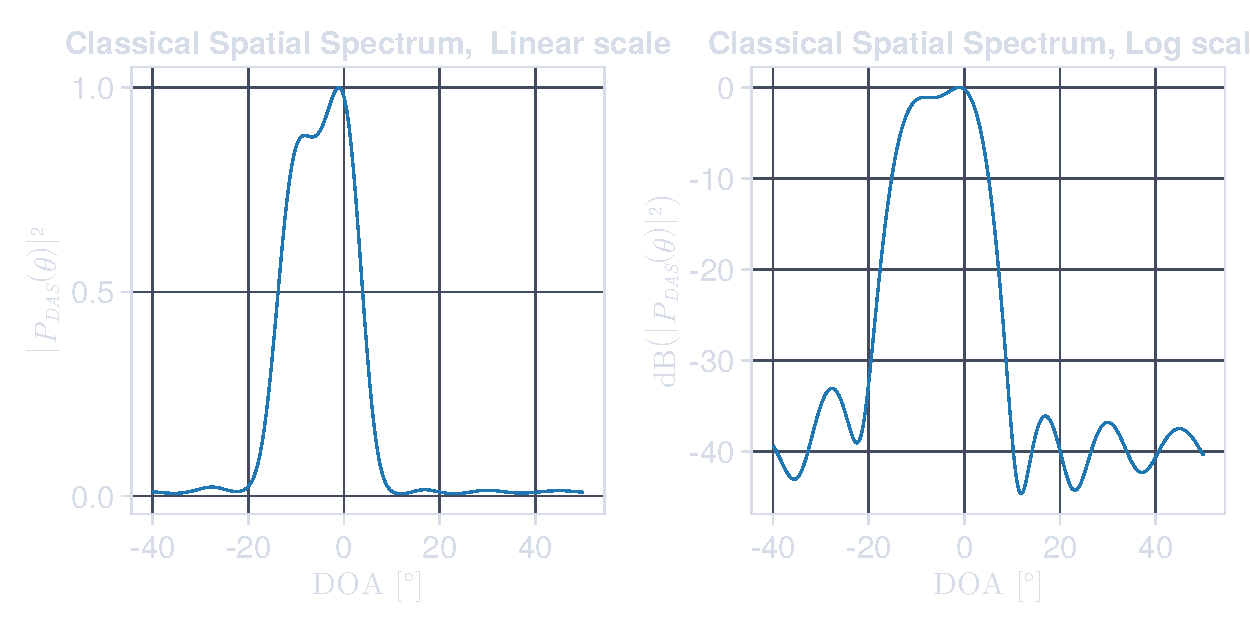
\includegraphics[width=\columnwidth]{"../b.pdf"}
            \end{figure}
        \end{column}
    \end{columns}
\end{frame}
% >>>

\begin{frame}[fragile] % <<< Estimate spatial spectrum with Capon's method
    \frametitle{Estimate spatial spectrum with Capon's method}
    Then we calculate it using minimum variance
    \begin{columns}
        \begin{column}{0.4\textwidth}
            \begin{itemize}
                \item Implementing the function is streight forward, following
                    the definition of Capon's method
            \end{itemize}
            \begin{jllisting}[gobble=16]
                P_CAP(θ) = 1 / (a(θ)'*inv(R)*a(θ))
                
                P_BF2 = @. abs(P_CAP(DOA))^2
                P_BF2 ./= maximum(P_BF2);
            \end{jllisting}
        \end{column}
        \begin{column}{0.6\textwidth}
            \begin{figure}
                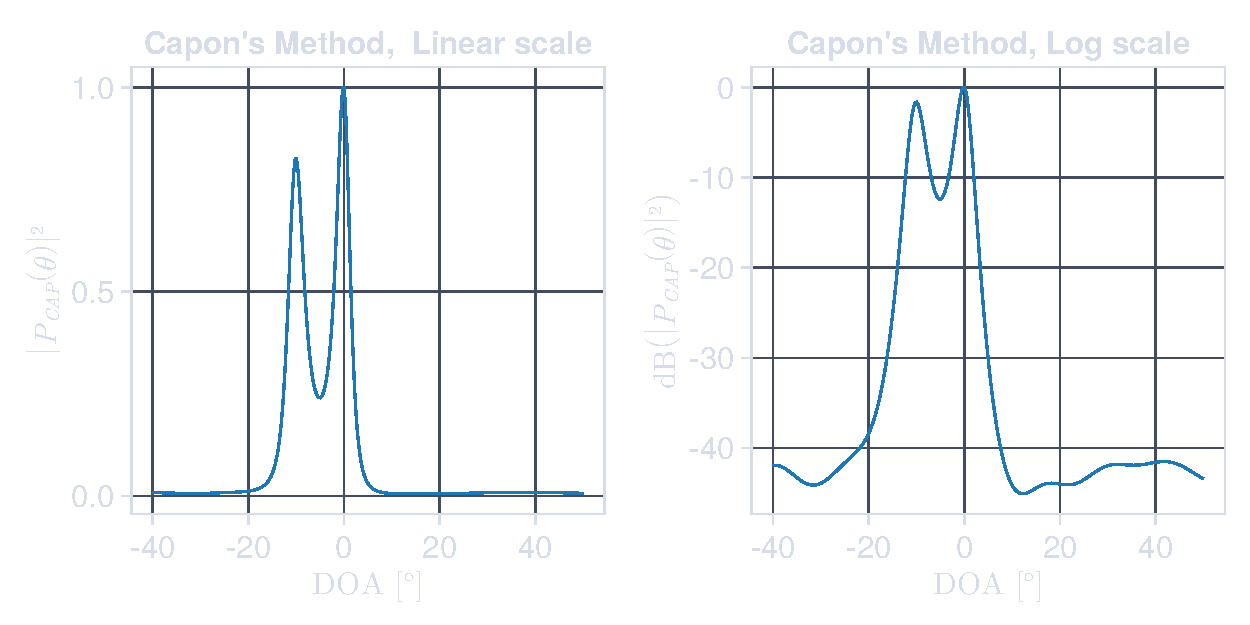
\includegraphics[width=\columnwidth]{"../c.pdf"}
            \end{figure}
        \end{column}
    \end{columns}
\end{frame}
% >>>

\begin{frame}[fragile] % <<< Eigenvalue distribution
    \frametitle{Eigenvalue distribution}
    We want to find the distribution of eigenvalues and plot them in descending
    order.
    \begin{columns}
        \begin{column}{0.5\textwidth}
            \begin{itemize}
                \item We decompose {\bf R} using \jlinl{eigvals} and \jlinl{eigvecs}.
                \item They are sorted in ascending order, so we reverse them inplace.
            \end{itemize}
            \begin{jllisting}[gobble=16]
                dd, V = eigvals(R), eigvecs(R);
                reverse!(dd); reverse!(V, dims=2);
            \end{jllisting}
        \end{column}
        \begin{column}{0.5\textwidth}
            \begin{figure}
                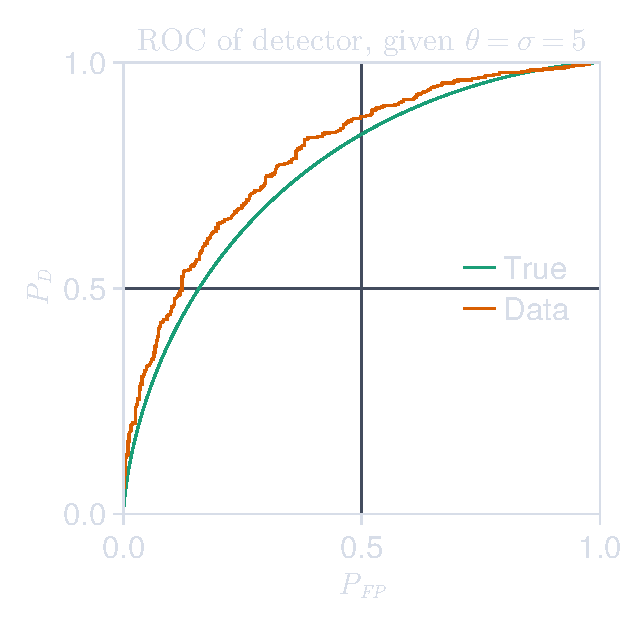
\includegraphics[width=\columnwidth]{"../d.pdf"}
            \end{figure}
        \end{column}
    \end{columns}
\end{frame}
% >>>

\begin{frame}[fragile] % <<< Spatial spectrum using MUSIC
    \frametitle{Spatial spectrum using MUSIC}
    We assume to know the number of sources is know (2) and we find the spatial
    spectrum using the MUSIC method.
    \begin{columns}
        \begin{column}{0.4\textwidth}
            \begin{itemize}
                \item Take all eigenvectors corresponding to noise space
                \item Make MUSIC
            \end{itemize}
            \begin{jllisting}[gobble=16]
                U = V[:, 3:end]
                Π = U*U'
                P_M(θ) = 1/(a(θ)'*Π*a(θ))

                P_BF3 = @. abs(P_M(DOA))^2
                P_BF3 ./= maximum(P_BF3);
            \end{jllisting}
        \end{column}
        \begin{column}{0.6\textwidth}
            \begin{figure}
                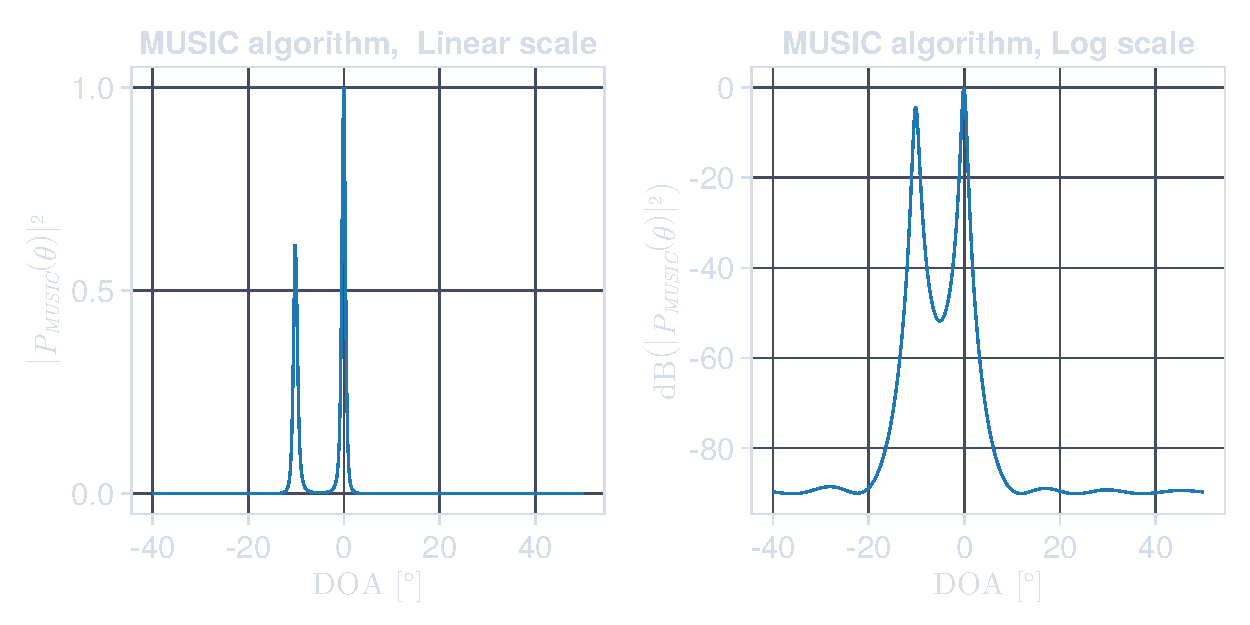
\includegraphics[width=\columnwidth]{"../e.pdf"}
            \end{figure}
        \end{column}
    \end{columns}
\end{frame}
% >>>

\begin{frame}[fragile] % <<< Spatial spectrum using Eigenvector method
    \frametitle{Spatial spectrum using Eigenvector method}
    Now we use the eigenvalues as weights in the MUSIC method. This gives the 
    Eigenvector method.
    \begin{columns}
        \begin{column}{0.4\textwidth}
            \begin{itemize}
                \item We construct a diagonal matrix of the Eigenvalues $\Lambda$
                    which serve as weights for the Eigenvectors.
            \end{itemize}
            \begin{jllisting}[gobble=16]
                U = V[:, 3:end]
                Λ⁻¹ = inv(diagm(dd[3:end]))
                P_EV(θ) = 1/(a(θ)'*U*Λ⁻¹*U'*a(θ))

                P_BF4 = @. abs(P_EV(DOA))^2
                P_BF4 ./= maximum(P_BF4);
            \end{jllisting}
        \end{column}
        \begin{column}{0.6\textwidth}
            \begin{figure}
                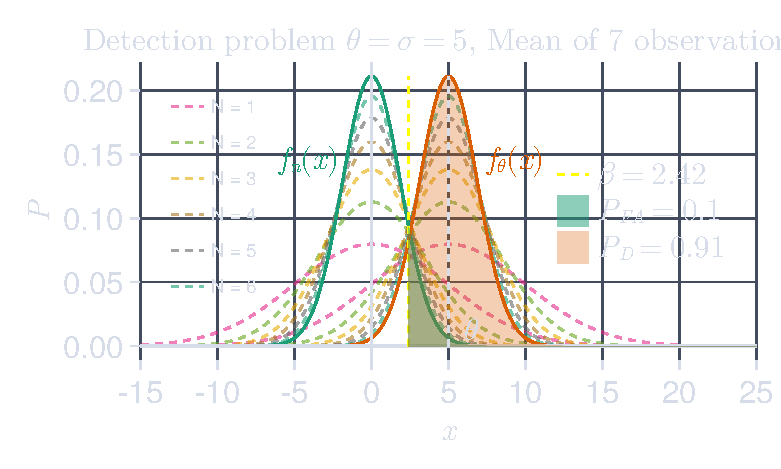
\includegraphics[width=\columnwidth]{"../f.pdf"}
            \end{figure}
        \end{column}
    \end{columns}
\end{frame}
% >>>

\begin{frame}[fragile] % <<< Incorrect estimation of number of sourcesIncorrect estimation of number of sources
    \frametitle{Incorrect estimation of number of sources}
    We now vary the number of sources we assume and plot both the MUSIC and the
    Eigenvector method.
    \begin{columns}
        \begin{column}{0.5\textwidth}
            \begin{itemize}
                \item We define a function that returns the spatial spectrum
                    given a number of sources
                \item We see that Eigenvector method given $N=0$ is identical to
                    Capon's method
            \end{itemize}
            \begin{jllisting}[gobble=16]
                function assume_sources(N)
                  U = V[:, N+1:end]
                  Λ⁻¹ = inv(diagm(dd[N+1:end]))
                  P0 = θ -> 1/(a(θ)'*U*U'*a(θ))
                  P1 = θ -> 1/(a(θ)'*U*Λ⁻¹*U'*a(θ))
                  return (
                    (@. abs(P0(DOA))^2) |> x -> x ./ maximum(x),
                    (@. abs(P1(DOA))^2) |> x -> x ./ maximum(x)
                  )
                end
            \end{jllisting}
        \end{column}
        \begin{column}{0.5\textwidth}
            \begin{figure}
                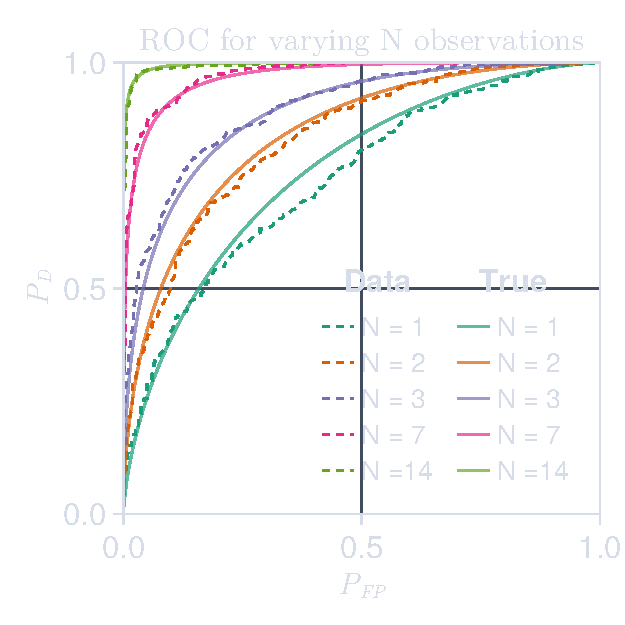
\includegraphics[width=\columnwidth]{"../g.pdf"}
            \end{figure}
        \end{column}
    \end{columns}
\end{frame}
% >>>

\begin{frame}[fragile] % <<< Coherent sources
    \frametitle{Coherent sources}
    Now we modify the \jlinl{generate_data.jl} to create coherent signals.
    \begin{columns}
        \begin{column}{0.5\textwidth}
            \begin{itemize}
                \item Code is identical to previous tasks, but uses different
                    data.
                \item There is $30\deg$ spearation between the sources compared
                    to only $10\deg$ in the previous data.
                \item We see the classical DAS is now better that all other
                    methods.
            \end{itemize}
        \end{column}
        \begin{column}{0.5\textwidth}
            \begin{figure}
                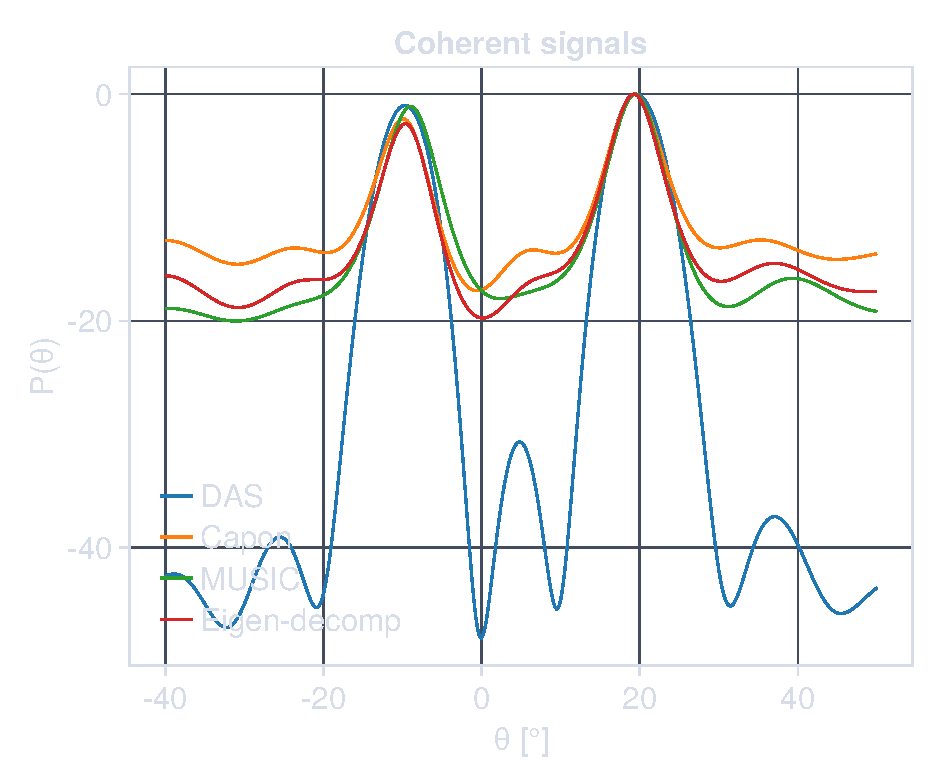
\includegraphics[width=\columnwidth]{"../i.pdf"}
            \end{figure}
        \end{column}
    \end{columns}
\end{frame}
% >>>

\end{document}
